\documentclass[a4paper]{article}
\title{Assignment 3}
\date{\textbf{Deadline}: 10 Dec 2023 - 11.59pm}
\author{name: Harkeerat Singh Sawhney, email: sawhnh@usi.ch}

%%%%%%%%%%%%%%%%%%%
% Packages
%%%%%%%%%%%%%%%%%%
\usepackage{palatino}
\usepackage{amsmath}
\usepackage{bm}
\usepackage{hyperref}
\usepackage{xcolor}
\usepackage{verbatim}
\usepackage{enumerate}
\usepackage{amsmath}
\usepackage{bm}
\usepackage{hyperref}
\usepackage{verbatim}
\usepackage{graphicx}
\usepackage{enumerate}
\usepackage{xcolor}
\usepackage{listings}
\usepackage{listings}
\usepackage{xcolor}
\usepackage{float}
\usepackage{amsmath}
\usepackage{amsmath, amssymb} % for math symbols and fonts
\usepackage{hyperref} % for hyperlinks
\usepackage{listings}
\usepackage{xcolor}
\usepackage{subcaption}
\usepackage{geometry}
\usepackage{hyperref}
\usepackage{array}
\usepackage{tikz-qtree}
\usepackage{booktabs}


%%%%%%%%%%%%%%%%%%%
% Commands
%%%%%%%%%%%%%%%%%%
\newcommand{\erre}{\mathbf{R}}


\begin{document}
\maketitle

\section{Language models with LSTM [90/100]}

\subsection{Data (20 points)}
\begin{enumerate}
    \item In this question we were asked to download the data and read it as a pandas data-frame. From which we were expected to filter only the news labeled with the category \textit{politics}. In Table \ref{tab:news} we can see the first 3 rows of the data-frame. The data-frame has 5 columns, namely \textit{Link}, \textit{Headline}, \textit{Category}, \textit{Short Description} and \textit{Authors}.
          \begin{table}[h]
              \centering
              \caption{First 3 rows of the data-frame}
              \label{tab:news}
              \resizebox{\textwidth}{!}{
                  \begin{tabular}{|c|p{3cm}|c|p{3cm}|p{2cm}|}
                      \hline
                      \textbf{Link}                                                                                               & \textbf{Headline}                                           & \textbf{Category} & \textbf{Short Description}                        & \textbf{Authors}       \\
                      \hline
                      \href{https://www.huffpost.com/entry/biden-us-forces...}{https://www.huffpost.com/entry/biden-us-forces...} & Biden Says U.S. Forces Would Defend Taiwan If...            & POLITICS          & President issues vow as tensions with China rise. &                        \\
                      \hline
                      \href{https://www.huffpost.com/entry/ukraine-festiva...}{https://www.huffpost.com/entry/ukraine-festiva...} & ‘Beautiful And Sad At The Same Time’: Ukrainian Festival... & POLITICS          & An annual celebration took on a different feel... & Jonathan Nicholson     \\
                      \hline
                      \href{https://www.huffpost.com/entry/europe-britain-...}{https://www.huffpost.com/entry/europe-britain-...} & Biden Says Queen's Death Left 'Giant Hole' For...           & POLITICS          & U.S. President Joe Biden, in London for the fu... & Darlene Superville, AP \\
                      \hline
                  \end{tabular}
              }
          \end{table}

    \item In this question we were asked for each title to be tokenized. This can be seen in the Table \ref{tab:headlines}.
          \begin{table}[H]
              \centering
              \caption{First 3 rows of the tokenized headlines}
              \label{tab:headlines}
              \begin{tabular}{|p{0.8\textwidth}|}
                  \hline
                  Biden says U.S. forces would defend Taiwan if China invaded \textless EOS\textgreater                                           \\
                  \hline
                  ‘Beautiful and sad at the same time’: Ukrainian cultural festival takes on a deeper meaning this year \textless EOS\textgreater \\
                  \hline
                  Biden says Queen's death left 'giant hole' for royal family \textless EOS\textgreater                                           \\
                  \hline
              \end{tabular}
          \end{table}
    \item In this question we were asked to create a named list called all\_tokens, where each element of the list is a vector of tokens from a headline. Then we were asked to create two dictionaries named word\_to\_id and id\_to\_word. The first one maps each word to a unique integer and the second one maps each integer to a unique word. Hence from this the top 5 most common words were EOS, biden, says, u.s., forces.
    \item In this question we were asked to create a dataset class which takes as input the list of tokenized sequences and the dictionary word-to-int. From there the output was supposed to be a tuble which has the first element as the indexes of all the words of the sentence except the last one, while at the other pair it is supposed to be the index of the last word of the sentence.

          Hence this was implemented by constructing a class called TextDataset which as it was asked takes both the tokenized sequences and the words to integer dictionary. It then converts the tokenized sequence to integers and then converts the list to an tensor. Lastly as specified it returns a tuple with the first one not including the first element while the second one is the last element.
    \item In this question we were asked to create a function called collate-fn(batch) which is supposed to pad the sequence with PAD until the maximum sequence size of the batch. This was implemented mainly by looking at Exercise 4, but how it is done is that we first unpack the batch, and then we use the pytorch function pad\_sequence to pad the sequence with PAD until the maximum sequence size of the batch. We do this for both the actual data and the targets. Lastly we return the padded data and the targets.
\end{enumerate}

\subsection{Model definition (20 points)}
In this question we were asked to implement an LSTM-based model where we were allowed to add whatever we liked, but we were supposed to have an Embedding at the beginning, and should use LTSM.

Firstly in the Model we have the initialization stage where we take all the parameters and initialize it to the local variables. We then create an Embedding Layer (as asked) which would transform the input into a vector of size embedding. We them implemented a LSTM Layer which is the core of our model. LSTM (Long Short-Term Memory) is a type of recurrent neural network (RNN) we can learn and remember patterns over time. We also added a Dropout Layer which is a regularization technique that prevents overfitting. We also then have a Fully Connected Layer which is used to transform the output of the LSTM to the size of the vocabulary. Lastly we have a Forward function which is used to pass the data through the model. We also have a hindi state which is used for the TBTT implementation. This is supposed to the same as init-state but it was used due to some bugs and simplicity.

\subsection{Evaluation - part 1 (10 points)}
\begin{itemize}
    \item In this question we were asked to implement the function random-sample-next which is supposed to act like the implementation of sampling strategy. This mean that this function is supposed to select the next token based on the probability distribution of the output of the model. This takes a probability distribution and samples a random token from it.
    \item In this question we were asked to implement the function sample-argmax which is supposed to be a greedy strategy. This means that this function is supposed to select the next token based on the probability distribution of the output of the model. This takes a probability distribution and selects the token with the highest probability.
    \item Lastly in this question we were asked to implement the function sample which takes as minima input a prompt, the model and one of the two function which we just implemented. We are supposed to use these parameters to generate a sequence of tokens until the model generates the EOS token.

          The way this was implemented was by first converting the prompt to a list of tokens. Then these list of tokens were converted to tensors, in which afterwards we were able to pass it through the model. We then enter a loop in which we generate each word at a time. It creates a probability distribution through softmax and then uses the sampler function to generate the next word. We then add the new generated word to the tokens and start the loop again. This is done until the EOS token is generated.
\end{itemize}

\subsection{Training (35 points)}
\begin{enumerate}
    \item In this question we are asked to implement the training loop which trains the model. We used the hyperparameters as mentioned in the remarks. We use the same optimizer as well as the same loss function as well which was mentioned.

          \begin{figure}[H]
              \centering
              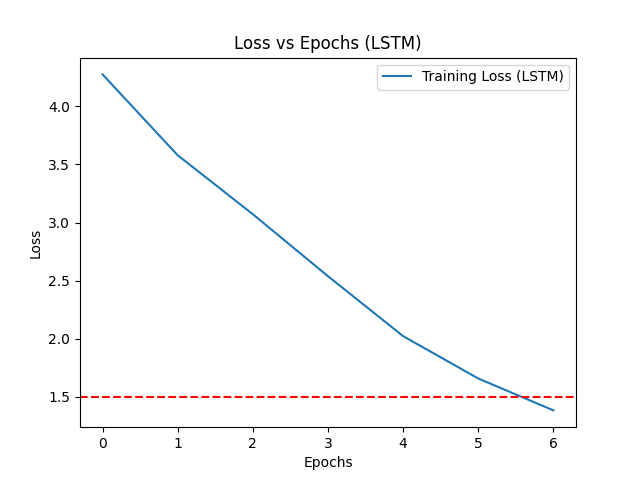
\includegraphics[width=0.8\textwidth]{"./plots/LSTM-training-loop-losses.png"}
              \caption{Training Loop Losses for LSTM}
              \label{fig:lstm-training-loop-losses}
          \end{figure}

          \begin{figure}[H]
              \centering
              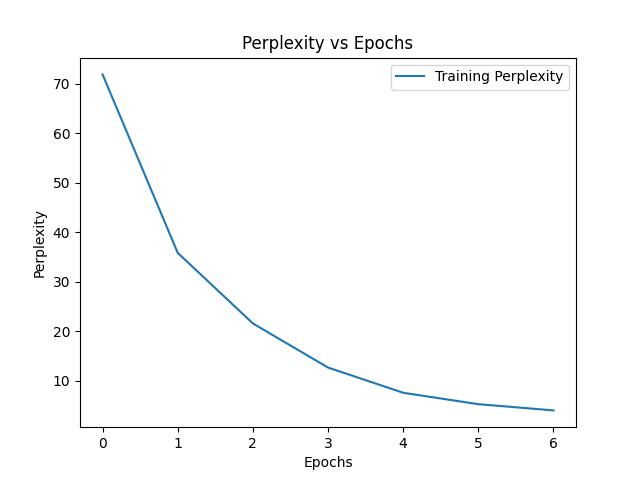
\includegraphics[width=0.8\textwidth]{"./plots/LSTM-training-loop-perplexities.png"}
              \caption{Training Loop Perplexities for LSTM}
              \label{fig:lstm-training-loop-perplexities}
          \end{figure}

          As it can be seen from the Figure \ref{fig:lstm-training-loop-losses} and Figure \ref{fig:lstm-training-loop-perplexities} that the losses and perplexities are decreasing as the epochs increase. The lose has also decreased bellow 1.5 as required and was also early stopped at epoch 6 to save time and computation power.

          Also the perplexity is also decreasing as the epochs increase and is also below 4 which indicates that the model is learning well. The sentences were also generated in different stages. Each sentence started with trump. The sentence generated at epoch 1 was \textit{trump to the the the the}. The sentence generated at epoch 3 was \textit{trump think elections}. Lastly the sentence generated at epoch 6 was \textit{trump to announce \$1 sanctions}.

    \item This implementation was tricky as we had to implement the TBTT training loop. The main difference between these two implementations are that the in the normal Training loop it is trained on the whole sequence at once. It initializes the model's state at the start of each sequence and does not carry it over between sequences. While for TBBTT we use the technique called Truncated backpropagattion Through Time (TBBTT), which breaks the sequence into smaller chunks and trains the whole model on these chunks. This approach is generally known to be more memory-efficient.

          For this implementation the same hyperparameters were used as mentioned in the remarks. The number of chunks was 15, and also the number of epochs was 10 to get the desired results. The losses and perplexities can be seen in Figure \ref{fig:lstm-tbtt-training-loop-losses} and Figure \ref{fig:lstm-tbtt-training-loop-perplexities} respectively. The losses and perplexities are decreasing as the epochs increase. However in this case at Epoch 6 it is lower than the normal Training Loop, and in the case of Perplexity it is much lower than the LSTM.
          \begin{figure}[H]
              \centering
              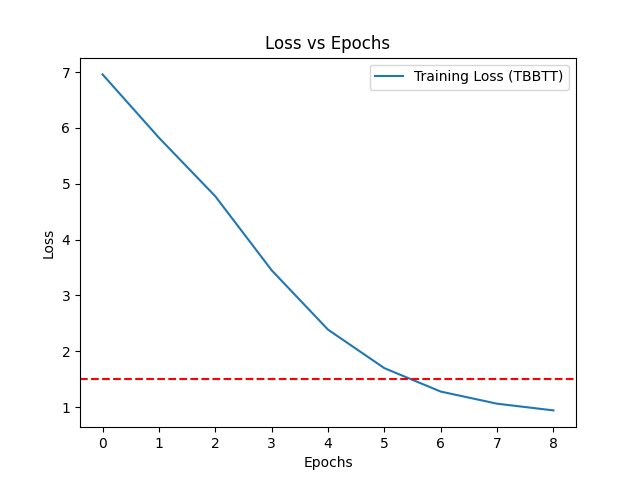
\includegraphics[width=0.8\textwidth]{"./plots/TBBTT-training-loop-losses.png"}
              \caption{Training Loop Losses for TBBTT}
              \label{fig:lstm-tbtt-training-loop-losses}
          \end{figure}

          \begin{figure}[H]
              \centering
              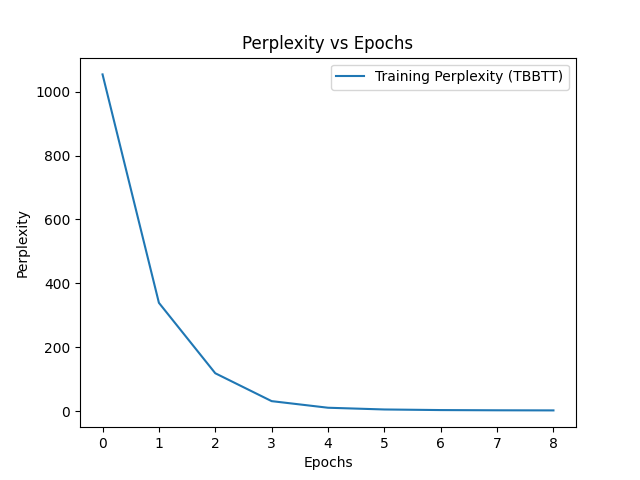
\includegraphics[width=0.8\textwidth]{"./plots/TBBTT-training-loop-perplexities.png"}
              \caption{Training Loop Perplexities for LSTM}
              \label{fig:lstm-tbtt-training-loop-perplexities}
          \end{figure}

          Also there were sentences generated which are as follows:
          \begin{itemize}
              \item \textit{earth to be a big of the union}
              \item \textit{earth for donald trump's travel ban}
              \item \textit{earth to help rebuild}
          \end{itemize}
\end{enumerate}

\subsection{Evaluation - part 2 (5 points)}
\begin{itemize}
    \item Bellow are the sentences generated by the LSTM and TBBTT models in sampling strategy.
          \begin{itemize}
              \item \textit{the president wants to criminalize a serious here's
                        where democrats}
              \item \textit{the president wants justice to fight the system white us}
              \item \textit{the president wants to make a debt ceiling down}

          \end{itemize}
    \item Bellow are the sentences generated by the LSTM and TBBTT models in greedy strategy.
          \begin{itemize}
              \item \textit{the president wants to drive more}
              \item \textit{the president wants to unilaterally disarm}
              \item \textit{the president wants to come in.}
          \end{itemize}
\end{itemize}

It is very interesting to see the results as I did not expect the titles to be generated in such a manner. Reading it does make the news sound vers absurd, but the sentences are properly formated together, and to an extend some do not makes sense, but some really do. One thing which I have noticed is that with sampling strategy the sentences are more diverse and different, while with greedy strategy the sentences are more similar to each other. Greedy strategy has more simpler and shorter sentences while sampling strategy has more complex and longer sentences.


\section{Questions [5 points]}
Character-level Byte-Pair Encoding (BPE) and WordPiece are two popular subword tokenization techniques which help out with handling the out-of-vocabulary words and improve the model generalization.

BPE starts with a vocabulary of the individual characters and iteratively it merges the most frequent pair of symbols to form new symbols. This is done until the desired vocabulary size has been reached. This is helpful, because in cases where there are rare and unseen words BPE is able to break down the words into subwords, which then can be searched in the vocabulary. This is also helpful in cases where there are misspelled words, as it is able to break down the words into subwords and then search for the subwords in the vocabulary.

Similar to BPE, WordPiece also starts with a vocabulary of the individual words. However the difference is in the merging process. In WordPiece the merging process is done greedily, which means that it merges the most frequent pair of symbols to form new symbols. This is done until the desired vocabulary size has been reached. This is helpful, because in cases where there are rare and unseen words WordPiece is able to break down the words into subwords, which then can be searched in the vocabulary.


\section{Technical Problems}
Since my GPU is not powerfull enough, I had to use Kaggle to train the models. However I have downloaded all the folders and files, so the code should still work fine as it worked in the Kaggle Notebook.
\end{document}
